\documentclass{article}
\usepackage{amsmath,amssymb,amsthm}
\usepackage{graphicx}
\usepackage[all]{xy}
\usepackage{tikz}
\newtheorem{proposition}{Proposition}
\newtheorem{example}{Example}
\title{Layout Cases}
\author{First Author \and Second Author\\ Some Institute}
\date{\today}
\begin{document}
\maketitle
\linespread{1.08}\selectfont

\section{One}
\begin{proposition}\label{prop:one}
Every $x$ satisfies $x = x$.
\end{proposition}\begin{proof}
Obvious.
\end{proof}

Some text before an example. \begin{example}\label{ex:mid:line}
An example that starts in the middle of a line.
\end{example} Text after the example on the same line.

\section{Two}
A diagram:
\[
\xymatrix{ A \ar[r]^f & B }
\]
See Proposition~\ref{prop:one} and Example~\ref{ex:mid:line}.

\begin{figure}[h]
\centering

\includegraphics[width=0.3\textwidth]{square.pdf}
\caption{A square.}
\end{figure}

\section{Three}
\begin{figure}[h]
\centering
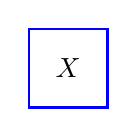
\begin{tikzpicture}
\draw[thick, blue] (0,0) rectangle (1,1);
\node at (0.5,0.5) {$X$};
\end{tikzpicture}
\caption{A picture.}
\end{figure}
Arrows: $A \xlongrightarrow{f} B$, $(a),\allowbreak(b)$.

Final words.
\end{document}
